\documentclass[10pt]{article}
\usepackage[spanish]{babel}
\usepackage[utf8]{inputenc}
\usepackage[T1]{fontenc}
\usepackage{graphicx}
\usepackage[export]{adjustbox}
\graphicspath{ {./images/} }
\usepackage{amsmath}
\usepackage{amsfonts}
\usepackage{amssymb}
\usepackage[version=4]{mhchem}
\usepackage{stmaryrd}
\usepackage{bbold}

\begin{document}
\section*{Geometría de Curvas y Superficies}
Trabajo grupal Marzo 2025\\

\includegraphics[max width=\textwidth, center]{2025_03_21_0cd0f59dd73209fa5cebg-1}

Universidad de Oviedo

\section*{Enunciado}
Un toro es la superficie de revolución generada por una circunferencia al girar alrededor de un eje situado en su mismo plano y que no la corta.\\
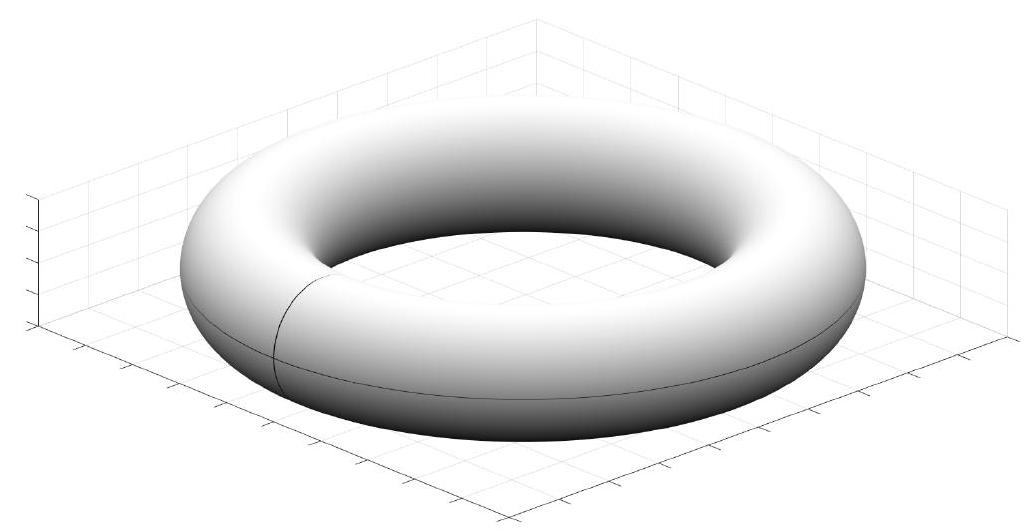
\includegraphics[max width=\textwidth, center]{2025_03_21_0cd0f59dd73209fa5cebg-2}

Figure 1: Parametrización de un toro en $\mathbb{R}^{3}$

Sean $a, b \in \mathbb{R}$ con $0<a<b$.\\
Consideremos el toro cuya curva generatriz es la circunferencia de centro en el punto ( $a, 0,0$ ) $y$ radio $b$ situada en el plano $y=0$. Dicha circunferencia gira alrededor del eje $z$.\\
(i) Usando como parámetros $u \in(0,2 \pi)$, ángulo de giro del punto inicial respecto del eje $x, y$ $v \in(0,2 \pi)$, ángulo de giro de dicho punto respecto del eje z, obtener una parametrización del toro, como superficie de revolución, de la forma

$$
\begin{aligned}
X: U=(0,2 \pi) \times(0,2 \pi) \subseteq \mathbb{R}^{2} & \longrightarrow \mathbb{R}^{3} \\
(u, v) & \longmapsto X(u, v)=(x(u, v), y(u, v), z(u, v))
\end{aligned}
$$

(ii) Con ayuda de dicha parametrización, obtener una ecuación cartesiana de la superficie generada, es decir, de modo que el toro se pueda expresar en la forma

$$
\mathbb{T}=\left\{(x, y, z) \in \mathbb{R}^{3}: F(x, y, z)=0\right\}
$$

noindent donde $F$ es una función que hay que determinar.\\
(iii) Determinar si $X$ es una carta del toro de clase $C^{k}(k \geq 1)$.\\
(iv) Determinar el plano tangente al toro $y$ el vector unitario normal en cada punto regular $p=X(q), q \in U$ del soporte $X(U)$


\end{document}